\chapter{Word embeddings}
In this chapter, we will discuss ways of representing text numerically, how we can create word embeddings and details around the word2vec technique from architectural choices to data preprocessing. At last, we will cover evaluation of word2vec models.

TODO: Change chapter introduction.

\section{Numerical representation of text}
Machine learning methods take in vectors (arrays of numbers) as input. When we want to work with text, we have to come up with some procedure for converting text into a vector, (i.e. vectorizing the text).
In this section, we will create some unique representation for words in a text, discuss one-hot encoding of words and the motivation behind creating word embeddings.

\subsection{Unique representation for each word}
\label{unique-representation-for-each-word}
A first strategy for vectorizing text could be to assign a unique number for each word in the text. We use the same order as the words appear in the text to assign a unique number. Furthermore, we define the number of unique words in the text to be the vocabulary size, denoted by $|V|$. We replace each word in the text with its respective number. Let us consider the following sentence
\begin{align}
    \text{the cat sat on the mat} \label{txt:num-rep-ex-sent-words}
\end{align}
\noindent
We convert the words into numbers based on the order they appear in the text, e.g., the $\mapsto$ 0, cat $\mapsto$ 1, sat $\mapsto$ 2, etc.
\begin{align}
    \text{0 1 2 3 0 4} \label{txt:num-rep-ex-sent}
\end{align}
We now have a numerical representation of the original sentence in $\ref{txt:num-rep-ex-sent-words}$ and may use it for machine learning modeling.

\noindent
There are some problems with this method, however.
\begin{itemize}
    \item The encoding of words into number is arbitrary (does not capture any relationship between words)
    \item Machine learning models might learn some natural ordering of the encodings, which can lead to bad results during inference. This is because the encoding of the words does not capture relationship between the words.
\end{itemize}

\noindent
In the next subsection, we will look at another method of encoding words, using one-hot encodings. We will also apply it to the example sentence in \ref{txt:num-rep-ex-sent-words}.

\subsection{One-hot encoded words}
One-hot encoding is a method for converting categorical data into numeric data. Essentially, we create a unique, sparse vector consisting of all zeros, except for the value at the index of the element of interest, which we set to one. For instance, if we have the words "north", "east", "south", "west", then their one-hot encodings could be
\begin{align}
    \text{north} \mapsto \begin{pmatrix}
    1\\
    0\\
    0\\
    0
    \end{pmatrix},
    \text{east} \mapsto \begin{pmatrix}
    0\\
    1\\
    0\\
    0
    \end{pmatrix},
    \text{south} \mapsto \begin{pmatrix}
    0\\
    0\\
    1\\
    0
    \end{pmatrix},
    \text{west} \mapsto \begin{pmatrix}
    0\\
    0\\
    0\\
    1
    \end{pmatrix}
\end{align}

\begin{definition}
Let $V = \left \{ w_1, w_2, ..., w_{|V|} \right \}$ denote the set of unique words in a text. Then, the one-hot encoding of a word, $e_{w_i}$, is defined as a $|V|$-dimensional vector of all zeros, except for the value at index $i$ which is one. \label{def:one-hot-encoding}
\end{definition}

\noindent
If we convert the numerical representation in \ref{txt:num-rep-ex-sent} using definition \ref{def:one-hot-encoding}, we get the following one-hot encoded vectors
\begin{align}
    \begin{pmatrix}
    1\\
    0\\
    0\\
    0\\
    0
    \end{pmatrix}
    \begin{pmatrix}
    0\\
    1\\
    0\\
    0\\
    0
    \end{pmatrix}
    \begin{pmatrix}
    0\\
    0\\
    1\\
    0\\
    0
    \end{pmatrix}
    \begin{pmatrix}
    0\\
    0\\
    0\\
    1\\
    0
    \end{pmatrix}
    \begin{pmatrix}
    1\\
    0\\
    0\\
    0\\
    0
    \end{pmatrix}
    \begin{pmatrix}
    0\\
    0\\
    0\\
    0\\
    1
    \end{pmatrix}
\end{align}
\noindent
We now have discarded the ordinal relationship of the numerical representation.

\noindent
There are some downsides with this approach as well, however.
\begin{itemize}
    \item As with the numerical representation in subsection \ref{unique-representation-for-each-word}, one-hot encoded vectors does not capture relationship between words.
    \item One-hot encoded vectors are sparse (meaning, most values are zero). Imagine if we had 1000 words in the vocabulary, then one would create a vector consisting of 99.9\% zeros. In practice, the vocabulary size is in the terms of $10^5$ to $10^7$ \cite{mikolov2013b}, e.g., by using one-hot encoded vector representations we are extremely inefficient in terms of space.
    \item One-hot encoded vectors are very high-dimensional (same as the number of words in the vocabulary, $|V|$).
\end{itemize}

\subsection{Word embeddings}
In contrast to the one-hot encoded vectors of words, word embeddings are low-dimensional dense vector representations. Word embeddings are typically learned from the data (e.g. texts) directly, whereas one-hot encoded vectors are statically defined. Due to the lower dimensionality of word embeddings, it packs more information about words into less space, thus being more efficient than one-hot encoded word vectors. Common choices for the dimensionality of word embeddings are ranging from 50 to 600 \cite{mikolov2013a}, depending on the amount of training data. We will take a look at a classic method of creating such word embeddings, called word2vec.

\section{Creating word embeddings (word2vec)}
Word2vec was first introduced by Mikolov et al. in 2013 \cite{mikolov2013a}. It is a family of techniques for learning dense and efficient vector representations of words. In the same year, Mikolov et al. introduced another paper which included several extensions that improved both the quality of the word embeddings and the training speed \cite{mikolov2013b}. In this section, we will go over the details of the original word2vec paper and the introduced extensions in the follow-up paper.

\subsection{Architectures}
The authors of the word2vec paper introduced two new log-linear models for learning distributed representations of words that try to minimize computational complexity, namely the continuous bag-of-words model (CBOW) and the continuous Skip-gram model. Both models achieve high quality word embeddings \cite{mikolov2013a} and share some core idea as to how one might create good vector representations of words. In this subsection, we will go through both models.

\subsubsection{Continuous bag-of-words model}
The continuous bag-of-words model (CBOW) tries to predict a target word given some context words around it. Essentially, we select a target word $w_t$, where $t$ is the index of the current target word in our training data, and a number $C$ denoting the number of words to the left and to the right of $w_t$. $C$ is also called the window size. By combining the projected word context vectors, we predict the target word $w_t$. This model is illustrated in \figref{fig:cbow-model}.

\begin{figure}[ht]
    \centering
    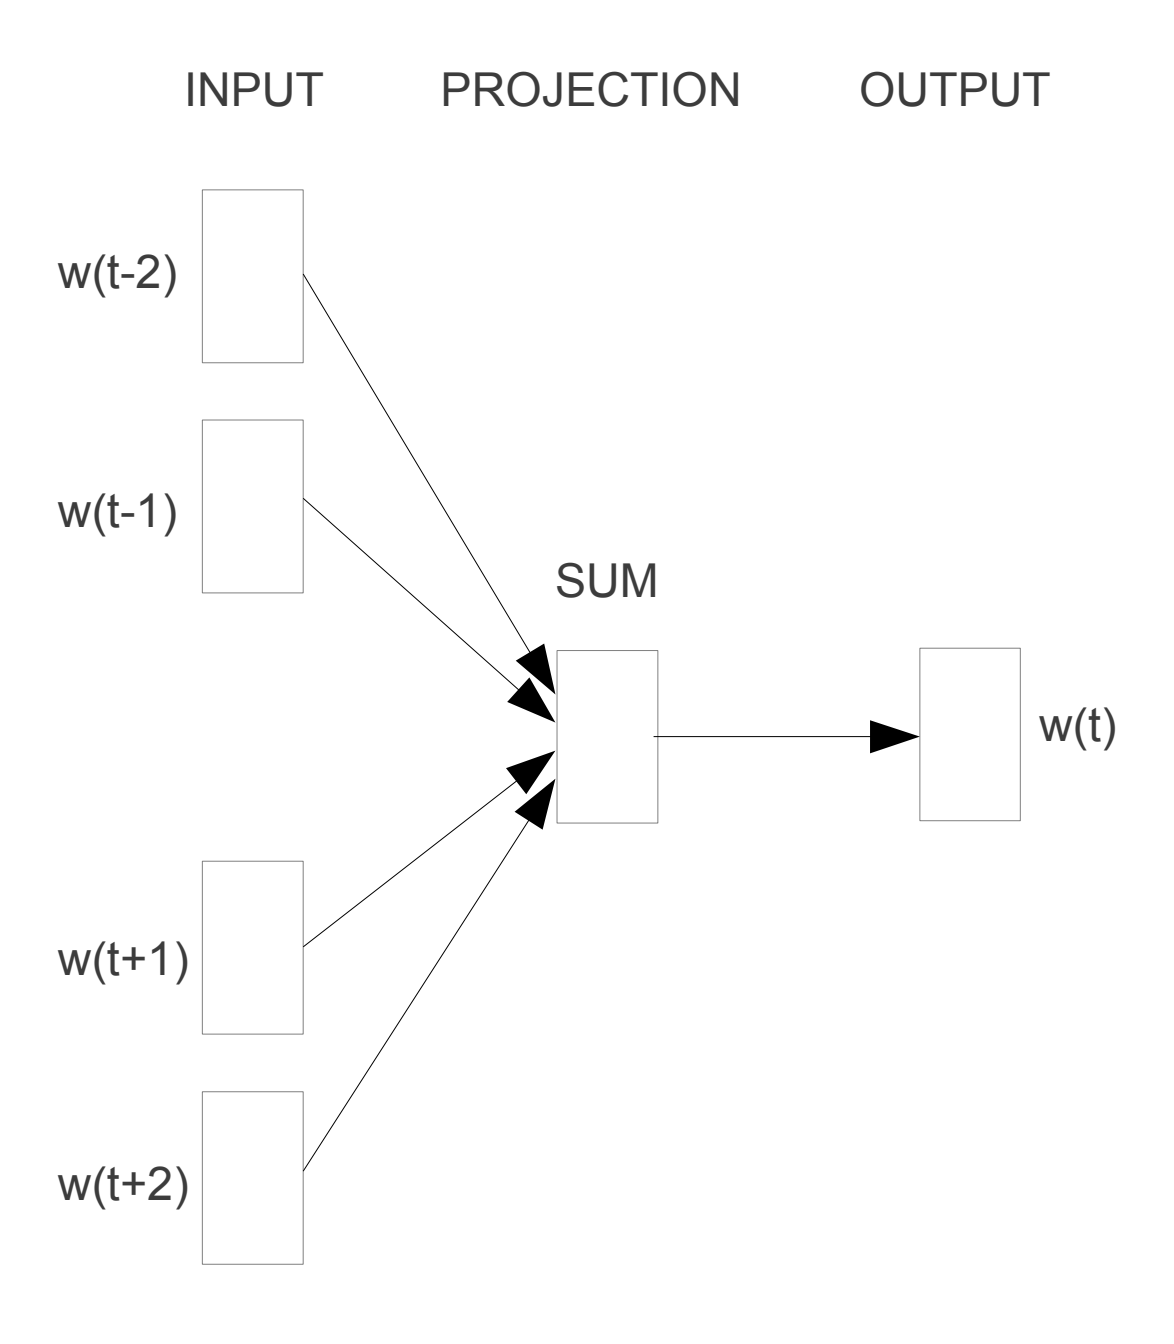
\includegraphics[width=8cm]{thesis/figures/cbow-mikolov-et-al-2013.png}
    \caption{CBOW architecture as illustrated by Mikolov et al. \cite{mikolov2013a}}
    \label{fig:cbow-model}
\end{figure}

\noindent
More formally, we are considering a sequence of $T$ training words $w_1, w_2, \ldots, w_T$. The words $w_t$ belong to some vocabulary $V$ consisting of $|V|$ unique words, $1 \leq t \leq T$. The models task is to maximize the average log probability of the word $w_t$ being sampled given the context words $w_{t-C}, \ldots, w_{t-1}, w_{t+1}, \ldots, w_{t+C}$. The objective of the CBOW model then becomes
\begin{align}
    \frac{1}{T} \sumlim{t=1}{T} \log p(w_t | w_{t-C}, \ldots, w_{t-1}, w_{t+1}, \ldots, w_{t+C})
    \label{eqn:cbow-objective-function}
\end{align}

\noindent
Through it is not clear from the original authors of word2vec \cite{mikolov2013a, mikolov2013b}, we typically use two weight matrices, $W$ and $W'$, when setting up the word2vec model \cite{rong2014word2vec}. The first weight matrix, $W$, is a $|V| \times D$ matrix, mapping the input word vectors (usually represented using one-hot encodings) to their internal embedding, where $|V|$ is the vocabulary size and $D$ is the number of dimensions in the hidden/projection layer. The second weight matrix, $W'$, is a $D \times |V|$ matrix mapping from the hidden/projection layer to the output prediction.

\subsubsection{Continuous Skip-gram model}
The continuous Skip-gram model is very similar to CBOW. In fact, the Skip-gram model tries to do the opposite; instead of predicting a target word given some context words, it tries to predict context words given some target word. The Skip-gram model is illustrated in \figref{fig:skip-gram-model}.

\begin{figure}[ht]
    \centering
    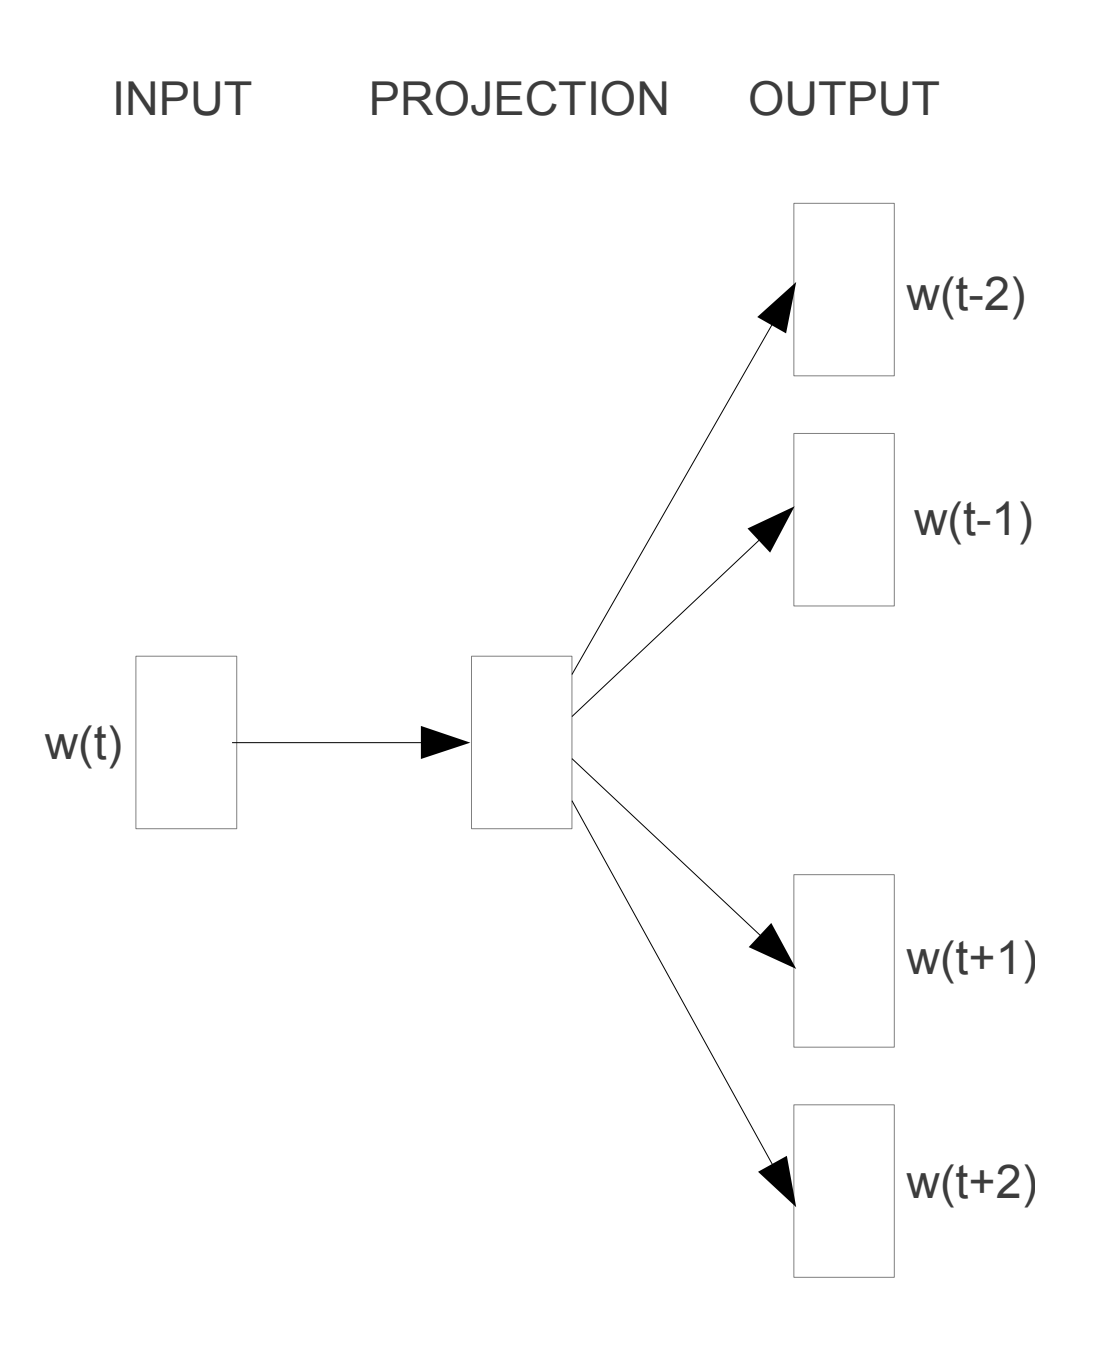
\includegraphics[width=8cm]{thesis/figures/skip-gram-mikolov-et-al-2013.png}
    \caption{The Skip-gram architecture as illustrated by Mikolov et al. \cite{mikolov2013a}}
    \label{fig:skip-gram-model}
\end{figure}

\noindent
As with the CBOW model, we have some target word $w_t$ with $C$ context words around it, $w_{t-C}, \ldots, w_{t-1}, w_{t+1}, \ldots, w_{t+C}$. The objective of the Skip-gram model \cite{mikolov2013b} then becomes
\begin{align}
    \frac{1}{T} \sumlim{t=1}{T} \sumlim{-C \leq j \leq C, j \neq 0}{} \log  p(w_{t+j} | w_t)
\end{align}

\noindent
Similar to CBOW, the Skip-gram model uses the two matrices $W$ and $W'$ for mapping from input to projection/hidden layer and projection/hidden layer to output respectively.

\noindent
Mikolov et al. reported that the Skip-gram model performed better than the CBOW model overall \cite{mikolov2013a}. For this reason and due to the scope of the masters thesis, we will stick to using the Skip-gram model throughout the thesis.

\subsection{Negative Sampling}

\noindent
In the Skip-gram model, we typically define $p(w_{t+j} | w_t)$ using the softmax function \cite{mikolov2013b} TODO: Reference softmax function?
\begin{align}
    p(w_{t+j} | w_t)
    &= \frac{\exp{ \left( \trans{v'_{t+j}} v_t \right) }} {\exp{  \sumlim{k=1}{|V|} \left( \trans{v'_k} v_t \right) }}
    \label{eqn:skip-gram-p-function}
\end{align}
where $v'_t$ and $v_t$ are the "input" and "output" vector representations of the word $w$, and $|V|$ is the number of words in the vocabulary. There are some downsides with this formulation, however. In practice, it becomes hard to compute since the summation in the denominator of equation \ref{eqn:skip-gram-p-function} depends on the number of words in the vocabulary, which is often large ($10^5 - 10^7$ terms) \cite{mikolov2013b}.

\noindent
To deal with the computational requirements of the original Skip-gram model, Mikolov et al. first showed how one might use hierarchical softmax \cite{mikolov2013b}. Hierarchical softmax is an efficient way of computing the softmax function; instead of evaluating $|V|$ words to compute the probability in equation \ref{eqn:skip-gram-p-function}, we only have to evaluate $\log \left( |V| \right)$ words \cite{mikolov2013b}.

\noindent
Following, Mikolov et al. introduce Negative sampling as an alternative to hierarchical softmax, which builds on the concept of distinguising a target word $w_t$ from a word randomly sampled from the vocabulary. In particular, we randomly sample words from the vocabulary using the unigram distribution raised to the power of $\alpha$ \cite{mikolov2013b}. The unigram distribution is a distribution for sampling a word at random from the vocabulary using the word occurrence counts, and the choice of raising it to the power of $\alpha = \frac{3}{4}$ was empirically found to be the best exponent. Furthermore, we will refer to this unigram distribution as the noise distribution $P_n(w)$ \cite{mikolov2013b}. Note that Negative sampling method can also be applied to CBOW in a similar manner \cite{mikolov2013b}.

\noindent
Before we can explain Negative sampling, we define the positive- and negative target-context pairs.
\begin{definition}
Given a vocabulary $V$, a target word $w_t$ and the target words contextual words $w_{t-C}, \ldots, w_{t-1}, w_{t+1}, \ldots, w_{t+C}$ for some window size $C$, we define a \textbf{positive target-context pair} to be the pair of the target word $w_t$ and a contextual word $w_{t+l}$, $-C \leq l \leq C, l \neq 0$, e.g., the pair $\left( w_t, w_{t+1} \right)$ for $l=1$. Furthermore, we define a \textbf{negative target-context pair} as the pair of the contextual word $w_{t+l}$ and a word $w_r$ randomly sampled from the noise distribution $P_n(w)$, e.g., the pair $\left( w_{t+l}, w_r \right)$.
\end{definition}

\noindent
In Negative sampling, we are only concerned with a subset of all the words in the vocabulary when computing the loss using the softmax function. For each word in the text we are training on, we create a positive target-context pair $\left( w_t, w_{t+l} \right)$, $-C \leq l \leq C, l \neq 0$. Furthermore, we generate $k$ negative target-context pairs for each word, where $k$ is in the range of $5-20$ for small training sets and $2-5$ for big training sets \cite{mikolov2013b}. We let $W_{np} = \left \{ w_j | j \in 1, \ldots, k \right \}$ be the set of $k$ negatively sampled words from the noise distribution $P_n(w)$. With these details in mind, the objective function of Negative sampling is \cite{mikolov2013b, rong2014word2vec}. TODO: Fix this equation, wronly stated at the moment.
\begin{align}
\log \sigma \left( \trans{w_t} w_{t+l} \right) + \sumlim{w_j \in W_{np}}{} \log \sigma \left( -\trans{w_j} w_{t+l} \right)
\label{eqn:negative-sampling-obj-func}
\end{align}
where $\sigma$ is the sigmoid function, e.g., $\sigma(z) = \frac{1}{1 + \exp{(-z)}}$. TODO: Reference sigmoid function?

\noindent
From equation \ref{eqn:negative-sampling-obj-func}, we see that we only have to compute for $(1 + k)$ words, which is a big improvement over computing for $|V|$ words (assuming that $|V|$ is much larger than $k$). Mikolov et al. also reports that by using Negative sampling, we increase the quality of the word embeddings \cite{mikolov2013b}.

\subsection{Subsampling of words}
When training a word2vec model, one usually has to train on big text corpora to achieve good quality of word embeddings \cite{mikolov2013a}. However, as the number of training words increase, the discrepancy between rare and frequent words increase as well. When using Negative sampling, we are sampling negative target-context pairs from the vocabulary, which depends on the unigram distribution. In English text corpora, words such as "the", "of", "is" can easily occur hundreds of millions of times and usually provide less information than more rare words \cite{mikolov2013b}. For this reason, we apply a simple, yet efficient subsampling scheme to counter the imbalance between rare and frequent words; before the text corpora is processed into target-context pairs, each word $w_t$ is discarded with the probability computed by the formula \cite{mikolov2013b, levy-etal-2015-improving}
\begin{equation}
    P_d(w_t) = 1 - \sqrt{\frac{t}{f(w_t)}}
\end{equation}
where $f(w_t)$ is the (relative) frequency of word $w_t$ and $t$ is a chosen threshold, usually around $10^{-5}$ \cite{mikolov2013b}.

\noindent
It should be noted, however, that in the source code of word2vec\footnote{\href{https://github.com/tmikolov/word2vec/blob/e092540633572b883e25b367938b0cca2cf3c0e7/word2vec.c\#L407}{word2vec.c at line 407 (of the original word2vec repository)}}, they use a slightly modified formula. We will use this formula when implementing word2vec.
\begin{align}
    P_d(w_t) = \frac{f(w_t) - t}{f(w_t)} - \sqrt{\frac{t}{f(w_t)}}
\end{align}

\subsection{Word2vec as an artificial neural network}
Typically in the literature, word2vec is presented using the equations \ref{eqn:cbow-objective-function}, \ref{eqn:skip-gram-p-function} and \ref{eqn:negative-sampling-obj-func}. We will, however, explain how to set word2vec up as an artificial neural network (ANN), in the sense that we will implement it later in the thesis. In particular, we will explain how to set up the Skip-gram model with negative sampling as an ANN. This ANN consists of three fully-connected layers of artificial neurons \cite{rong2014word2vec} and is illustrated in \figref{fig:word2vec-skip-gram-negative-sampling}.

\begin{figure}[ht]
    \centering
    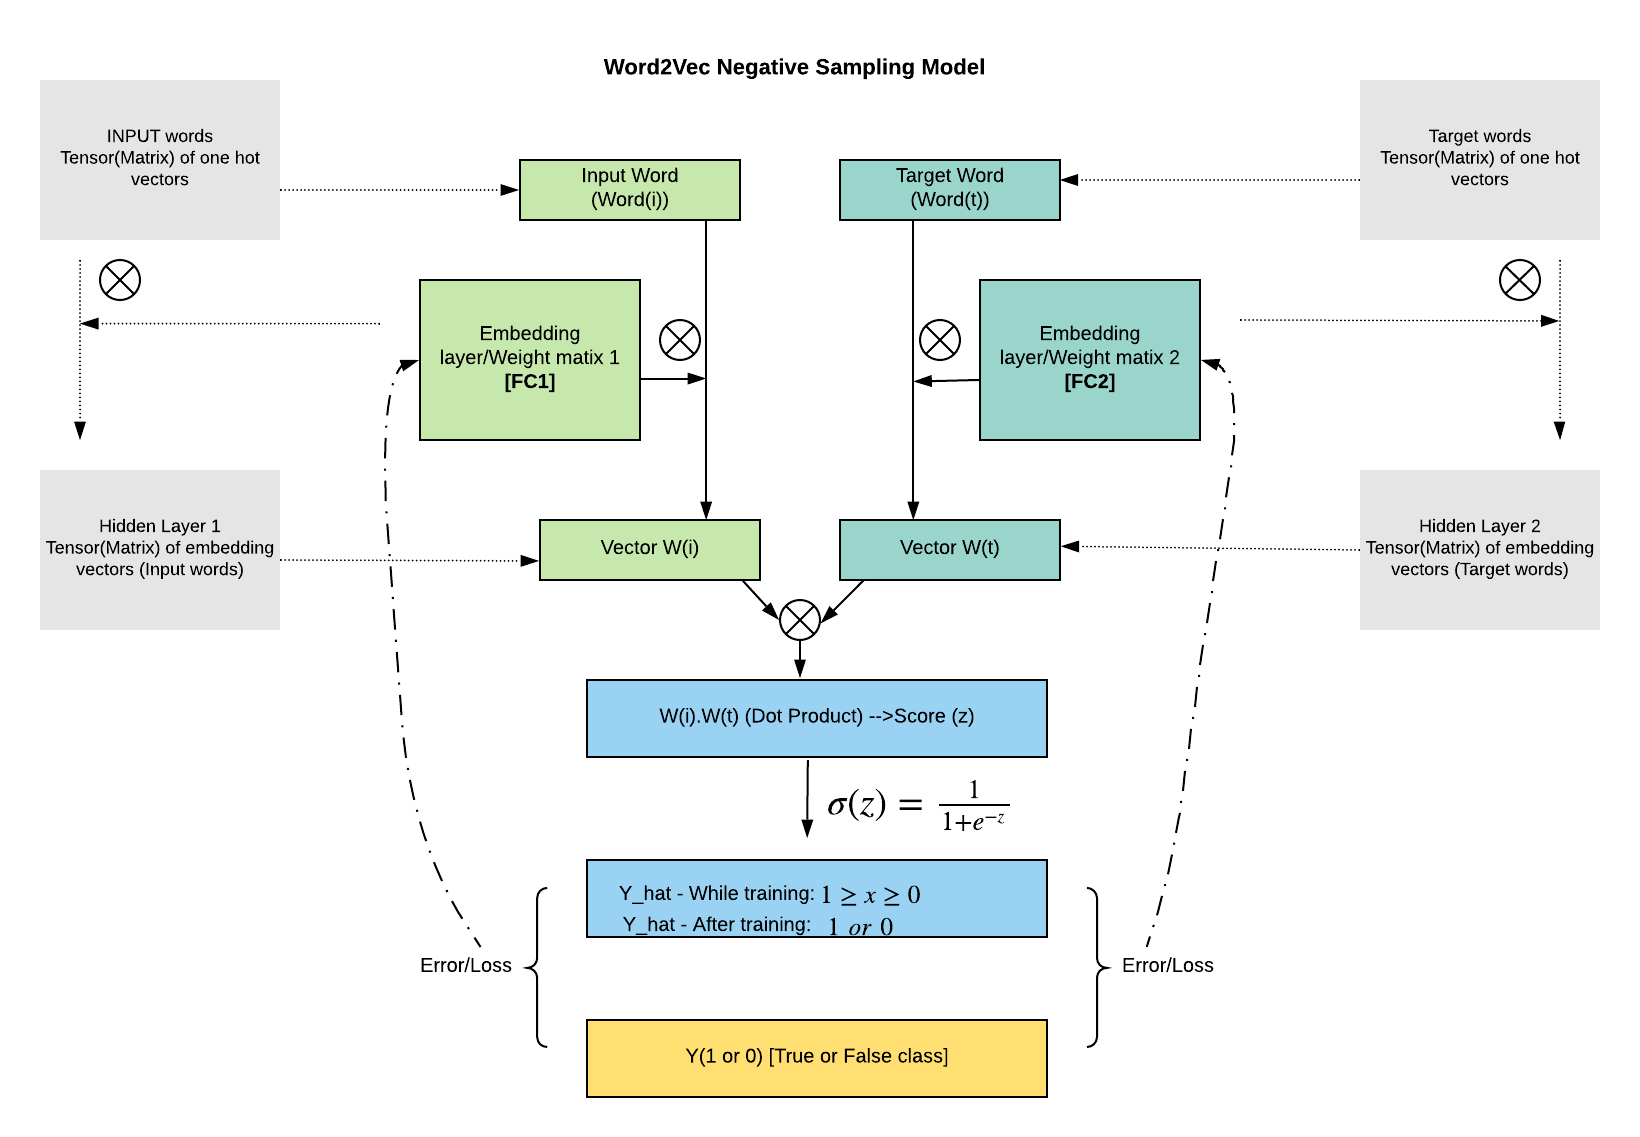
\includegraphics[width=12cm]{thesis/figures/word2vec-skip-gram-negative-sampling.png}
    \caption{TODO: Replace with TikZ illustration}
    \label{fig:word2vec-skip-gram-negative-sampling}
\end{figure}

\noindent
TODO: How to set it up, target vs context embedding, etc.

\section{Training a word2vec model}
TODO: Data preprocessing, Tensorflow, hyperparameters, etc.

\section{Evaluating a word2vec model}
TODO: Semantic and syntactic relations